\documentclass[11pt,a4paper]{article}
\usepackage{geometry}         
\geometry{a4paper}                   
\usepackage{graphicx}
\usepackage{amssymb}
\usepackage{epstopdf}
\usepackage{fancyhdr}
\usepackage[version=3]{mhchem}
\usepackage{caption}
\usepackage{float}
\usepackage{lastpage}
\usepackage{multirow}
\usepackage[titles]{tocloft}

%macros
\newcommand{\mshorttitle}{\sectionmark}
\newcommand{\mlongtitle}{Summary of Observation Data}

\newcommand{\mstudent}{David Ding, Jason Liu, Patrick Rall}
\newcommand{\mclass}{Team 2 - ``Bene Gesserit"}
\newcommand{\masteroid}{Asteroid: 1951 LICK}
\newcommand{\mschool}{SSP Westmont 2011}

\newcommand{\mversioning}{Rendered \today}

%header
\pagestyle{fancy}


\lhead{\mlongtitle}
\rhead{Team 2 - ``Bene Gesserit"}

%\lfoot{Page \thepage\ of \pageref{LastPage}}
\cfoot{}
\rfoot{\mversioning} 

\renewcommand{\headrulewidth}{0.4pt}
\renewcommand{\footrulewidth}{0.4pt}

%meta
\title{\mlongtitle}
\author{\mclass\\ \masteroid\\ \mschool}
\date{\mversioning}                                           

\begin{document}

\maketitle
\thispagestyle{empty}
\pagestyle{fancy}

%format
\widowpenalty=300
\clubpenalty=300

\setcounter{tocdepth}{2}
\setcounter{secnumdepth}{0}

\vspace{-12mm}

\tableofcontents
\clearpage


\newcommand{\rightascension}{$\alpha$}
\newcommand{\declination}{$\delta$}
\newcommand{\azimuth}{$A$}
\newcommand{\elevation}{$h$}
\newcommand{\hourangle}{$HA$}
\newcommand{\longitude}{$l$}
\newcommand{\latitude}{$\phi$}

\newcommand{\degrees}{$^{\circ}$}

%content
\section{List of Observations}

\begin{center}
\begin{tabular}{| c |  c | c | c | c | }
\hline
 Date (UT) &  \# series &  \#  imgs & Telescope & Sync Star \\ \hline \hline
 Series \# & JD & Filter & $\alpha_{\text{asteroid}}$  & $\delta_{\text{asteroid}}$   \\ \hline
\multicolumn{5}{|c|}{...} \\ \hline
\multicolumn{1}{c}{} \\[-2.5mm] \hline
July 1, 2011  & 3 & 15 & Meade LX200 14'' & Cor Coroli \\ \hline \hline
Series 1-3 & \multicolumn{4}{c|}{Omitted due to bad image quality}  \\  \hline
\multicolumn{1}{c}{} \\[-2.5mm]  \hline
July 3, 2011  & 3 & 15 & DFM 24'' & Arcturis \\ \hline \hline 
Series 1 & 2455745.73395 & Clear & 11h 34m 58.959$\pm$0.0294s & 40\degrees \space 39' 40.31$\pm$0.158'' \\ \hline
Series 2 & 2455745.74350 & Clear & 11h 35m 0.545$\pm$0.0657s & 40\degrees \space 39' 29.90$\pm$0.474'' \\ \hline 
Series 3 &\multicolumn{4}{|c|}{Omitted due to bad image quality} \\ \hline
\multicolumn{1}{c}{} \\[-2.5mm] \hline
July 8, 2011  & 4 & 28 & Meade LX200 14'' & Phecda \\ \hline \hline 
Series 1 &\multicolumn{4}{|c|}{Images are of wrong part of sky} \\ \hline
Series 2 & 2455750.72996 & Clear & 11h 50m 33.267$\pm$0.0139s & 39\degrees \space 3' 26.37$\pm$0.102'' \\ \hline 
Series 3 & 2455750.73822 & Clear& 11h 50m 34.834$\pm$0.0113s & 39\degrees \space 3' 16.64$\pm$0.143'' \\ \hline
Series 4 & 2455750.74774 & Clear & 11h 50m 36.644$\pm$0.00909s & 39\degrees \space 3' 4.32$\pm$0.170'' \\ \hline 
\multicolumn{1}{c}{} \\[-2.5mm]  \hline
July 10, 2011  & 3 & 21 & Meade LX200 14'' & Phecda \\ \hline \hline
Series 1 & 2455752.68928 & Clear & 11h 56m 37.351$\pm$0.0154s & 38\degrees \space 23' 33.02$\pm$0.150'' \\ \hline 
Series 2 & 2455752.70592  & Clear & 11h 56m 40.336$\pm$0.0113s & 38\degrees \space 23' 13.08$\pm$0.0921'' \\ \hline 
Series 3 & 2455752.71975 & Clear & 11h 56m 42.870$\pm$0.0104s & 38\degrees \space 22' 52.39$\pm$0.0682'' \\ \hline 
\multicolumn{1}{c}{} \\[-2.5mm]  \hline
July 16, 2011 & 5 & 25 & Meade LX200 14'' & Phecda \\ \hline \hline
Series 1 & 2455758.69142 & V-Filter & \multicolumn{2}{|c|}{Apparent magnitude $\approx$ 16.62} \\ \hline
Series 2 & 2455758.69609 & Clear & 12h 15m 3.471$\pm$0.0193s & 36\degrees \space 13' 55.36$\pm$0.185'' \\ \hline 
Series 3 & 2455758.70920 & Clear & 12h 15m 5.936$\pm$0.0259s & 36\degrees \space 13' 37.40$\pm$0.125'' \\ \hline 
Series 4 & 2455758.71939 & Clear & 12h 15m 7.671$\pm$0.0153s & 36\degrees \space 13' 22.93$\pm$0.117'' \\ \hline 
Series 5 & 2455758.72524 & Clear & 12h 15m 8.724$\pm$0.0253s & 36\degrees \space 13' 15.39$\pm$0.0949'' \\ \hline 
\multicolumn{1}{c}{} \\[-2.5mm]  \hline
July 19, 2011 & 4 & 28 & Meade LX200 14'' & Phecda \\ \hline \hline
Series 1 & 2455761.67834 & Clear & 12h 24m 7.855$\pm$0.0157s & 35\degrees \space 5' 27.33$\pm$0.190'' \\ \hline 
Series 2 & 2455761.69353 & Clear & 12h 24m 10.630$\pm$0.0207s & 35\degrees \space 5' 5.40$\pm$0.180'' \\ \hline 
Series 3 & 2455761.70952 & Clear & 12h 24m 13.432$\pm$0.0186s & 35\degrees \space 4' 43.58$\pm$0.172'' \\ \hline 
Series 4 & 2455761.72245 & Clear & 12h 24m 15.831$\pm$0.0195s & 35\degrees \space 4' 25.11$\pm$0.214'' \\ \hline 
\multicolumn{1}{c}{} \\[-2.5mm]  \hline
July 25, 2011 & 5 & 6 & Meade LX200 14'' & Phecda \\ \hline \hline
Series 1 & 2455767.690456 & Clear & 12h 42m 14.360$\pm$0.0427s & 32\degrees \space 39' 39.14$\pm$0.192'' \\ \hline 
Series 2 & 2455767.698177 & V-Filter & \multicolumn{2}{|c|}{Apparent magnitude $\approx$ 17.15} \\ \hline
\end{tabular}
\end{center}

Note: $\alpha$ and $\delta$ of the stars are taken from the NOMAD database whenever available, even though they are identified by their names within GSC and UCAC3 databases.

%%%%%%%%%%%%%%%%%%%%%%%%%%%%%%%%%%%%%%%%%%%%%%%%%%%%%%%%%%%%%%%%%%%%%%
%%%%%%%%%%%%%%%%%%%%%%%%%%%%%%    JUL 3     %%%%%%%%%%%%%%%%%%%%%%%%%%%%%%%%%

\clearpage
\section{July 3, 2011}
\subsection{Series 1}
\begin{center}
\begin{tabular}{| c |  c | c | c | }
\hline
JD & UT & \# images & Filter \\ \hline
2455745.73395 & 05h 36m 53.3s & 5 & Clear \\ \hline
\end{tabular}
\end{center}
\begin{center}
\begin{tabular}{| c |  c | c | c | }
\hline
 $x^{\text{asteroid}}_{\text{pixel}}$ & $y^{\text{asteroid}}_{\text{pixel}}$  & $\alpha_{\text{asteroid}}$ & $\delta_{\text{asteroid}}$ \\ \hline
423.333  & 322.288  & 11h 34m 58.959$\pm$0.0294s & 40\degrees \space 39' 40.31$\pm$0.158'' \\ \hline
\end{tabular}
\end{center}

\begin{figure}[h!]
  \centering
   %%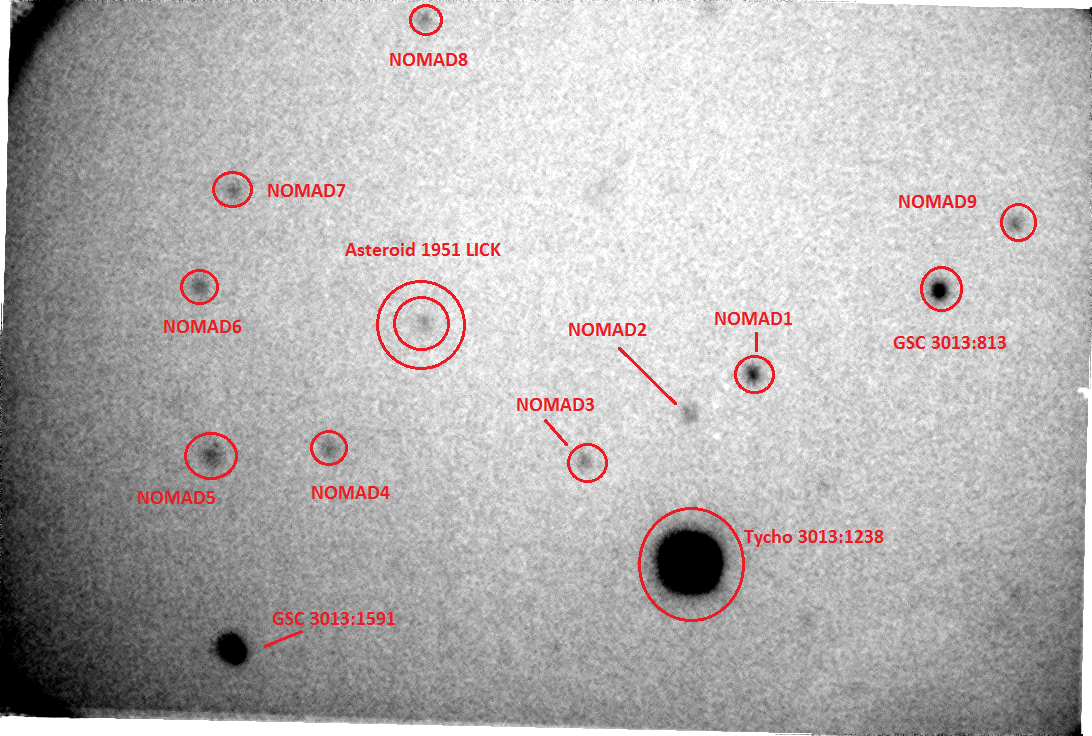
\includegraphics[width=\textwidth]{LSPR_annotated_images/Jul3Series1.png}
\end{figure}

Image quality from the 24'' telescope is surprisingly low. This is probably due bad focusing. Note the frost in the corners. However, the asteroid is neatly encircled by various usable reference stars.

\begin{center}
\begin{tabular}{| c |  c | c | c | c |  }
\hline
Star &  $x^{\text{star}}_{\text{pixel}}$ & $y^{\text{star}}_{\text{pixel}}$  & $\alpha_{\text{star}}$ &  $\delta_{\text{star}}$ \\ \hline \hline
GSC 3013:1238 & 693.189 & 563.466 & 11h 34m 47.229 $\pm 0.0442$s & 40\degrees \space 37' 04.81$\pm 0.0268$'' \\ \hline
GSC 3013:1591 &\multicolumn{4}{|c|}{Omitted due to background gradient} \\ \hline
GSC 3013:813 & 938.739 & 290.181 & 11h 34m 33.26 $\pm 0.0237$s & 40\degrees \space 39' 20$\pm 0.0814$'' \\ \hline
NOMAD1 & 752.345 & 373.849 & 11h 34m 43.04 $\pm 4.32\cdot 10^{-3}$s & 40\degrees \space 38' 47.12$\pm 0.156$'' \\ \hline
NOMAD2 &\multicolumn{4}{|c|}{Omitted to bad image quality} \\ \hline
NOMAD3 & 583.678 & 461.146 & 11h 34m 51.90 $\pm 0.0327$s & 40\degrees \space 38' 10.41$\pm 0.0333$'' \\ \hline
NOMAD4 & 328.643 & 448.533 & 11h 35m 04.42 $\pm 0.0312$s & 40\degrees \space 38' 36.38$\pm$ 0.00994'' \\ \hline
NOMAD5 & 211.086 & 455.347 & 11h 35m 10.33 $\pm 0.0266$s & 40\degrees \space 38' 41.17$\pm 0.0562$'' \\ \hline
NOMAD6 & 199.102 & 286.225 & 11h 35m 9.80 $\pm 0.0106$s & 40\degrees \space 40' 17.12$\pm 0.0125$'' \\ \hline
NOMAD7 & 232.423 & 190.196 & 11h 35m 7.54 $\pm 0.00672$s & 40\degrees \space 41' 8.77$\pm 0.137$'' \\ \hline
NOMAD8 & 423.324 & 19.078 & 11h 34m 57.03 $\pm 0.0246$s & 40\degrees \space 42' 30.58$\pm 0.0964$'' \\ \hline
NOMAD9 & 1014.671 & 223.004 & 11h 34m 29.10 $\pm 0.00529$s & 40\degrees \space 39' 52.17$\pm 0.0233$'' \\ \hline
\end{tabular}
\end{center}

%%%%%%%%%%%%%%%%%%%%%%%%%%%%%%%%%%%%%%%%%%%%%%%%%%%%%%%%%%%%%%%%%%%%%%

\clearpage
\section*{July 3, 2011}
\subsection{Series 2}
\begin{center}
\begin{tabular}{| c |  c | c | c | }
\hline
JD & UT & \# images & Filter \\ \hline
2455745.74350 & 05h 50m 38.4s & 5 & Clear \\ \hline
\end{tabular}
\end{center}
\begin{center}
\begin{tabular}{| c |  c | c | c | c |  c |  c |  c | }
\hline
$x^{\text{asteroid}}_{\text{pixel}}$ & $y^{\text{asteroid}}_{\text{pixel}}$  & $\alpha_{\text{asteroid}}$ & $\delta_{\text{asteroid}}$ \\ \hline \hline
384.414  & 347.392  & 11h 35m 0.545$\pm$0.0657s & 40\degrees \space 39' 29.90$\pm$0.474'' \\ \hline 
\end{tabular}
\end{center}

\begin{figure}[h!]
  \centering
   %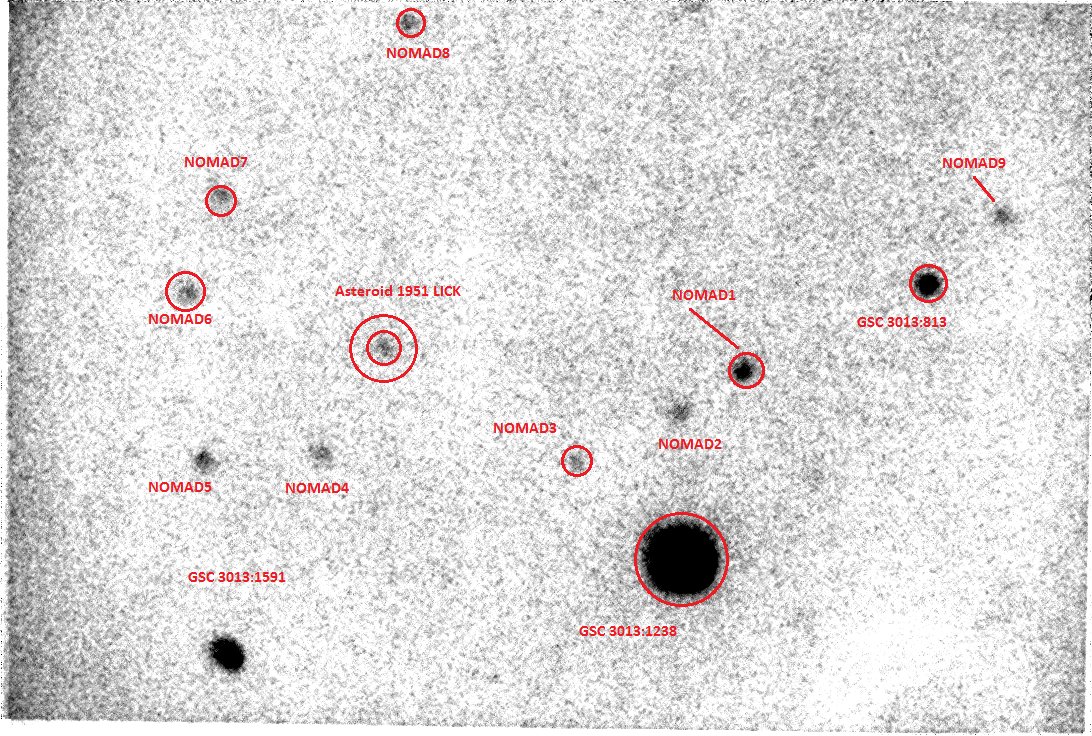
\includegraphics[width=\textwidth]{LSPR_annotated_images/Jul3Series2.png}
\end{figure}


\begin{center}
\begin{tabular}{| c |  c | c | c | c |  c | }
\hline
Star &  $x^{\text{star}}_{\text{pixel}}$ & $y^{\text{star}}_{\text{pixel}}$  & $\alpha_{\text{star}}$ &  $\delta_{\text{star}}$ \\ \hline \hline
GSC 3013:1238 & 687.924 & 561.721 & 11h 34m 47.229 $\pm 0.0824$s & 40\degrees \space 37' 04.81$\pm 0.272$'' \\ \hline
GSC 3013:1591 &\multicolumn{4}{|c|}{Omitted as location contains many stars} \\ \hline
GSC 3013:813 & 927.411 & 284.064 & 11h 34m 33.26 $\pm 0.0223$s & 40\degrees \space 39' 20$\pm 0.29$'' \\ \hline
NOMAD1 & 742.878 & 370.526 & 11h 34m 43.04 $\pm 0.0135$s & 40\degrees \space 38' 47.12$\pm 0.0665$'' \\ \hline
NOMAD2 &\multicolumn{4}{|c|}{Omitted due to bad image quality} \\ \hline
NOMAD3 & 574.685 & 461.697 & 11h 34m 51.90 $\pm 0.0927$s & 40\degrees \space 38' 10.41$\pm 0.0948$'' \\ \hline
NOMAD4 &\multicolumn{4}{|c|}{Omitted due to bad image quality} \\ \hline
NOMAD5 &\multicolumn{4}{|c|}{Omitted due to bad image quality} \\ \hline
NOMAD6 & 187.730 & 291.800 & 11h 35m 9.80 $\pm 0.0469$s & 40\degrees \space 40' 17.12$\pm 0.219$'' \\ \hline
NOMAD7 & 221.256 & 194.855 & 11h 35m 7.54 $\pm 0.0581$s & 40\degrees \space 41' 8.77$\pm 0.176$'' \\ \hline
NOMAD8 & 407.455 & 22.526 & 11h 34m 57.03 $\pm 0.00797$s & 40\degrees \space 42' 30.58$\pm 0.384$'' \\ \hline
NOMAD9 &\multicolumn{4}{|c|}{Omitted due to bad image quality} \\ \hline
\end{tabular}
\end{center}



%%%%%%%%%%%%%%%%%%%%%%%%%%%%%%%%%%%%%%%%%%%%%%%%%%%%%%%%%%%%%%%%%%%%%%
%%%%%%%%%%%%%%%%%%%%%%%%%%%%%%    JUL 8     %%%%%%%%%%%%%%%%%%%%%%%%%%%%%%%%

\clearpage
\section{July 8, 2011}
\subsection{Series 2}
\begin{center}
\begin{tabular}{| c |  c | c | c | }
\hline
JD & UT & \# images & Filter \\ \hline
2455750.72996 & 05h 31m 08.5s & 7 & Clear \\ \hline
\end{tabular}
\end{center}
\begin{center}
\begin{tabular}{| c |  c | c | c | c |  c |  c |  c | }
\hline
$x^{\text{asteroid}}_{\text{pixel}}$ & $x^{\text{asteroid}}_{\text{pixel}}$  & $\alpha_{\text{asteroid}}$ & $\delta_{\text{asteroid}}$ \\ \hline \hline
481.898  & 63.322  & 11h 50m 33.267$\pm$0.0139s & 39\degrees \space 3' 26.37$\pm$0.102'' \\ \hline 
\end{tabular}
\end{center}

\begin{figure}[h!]
  \centering
%   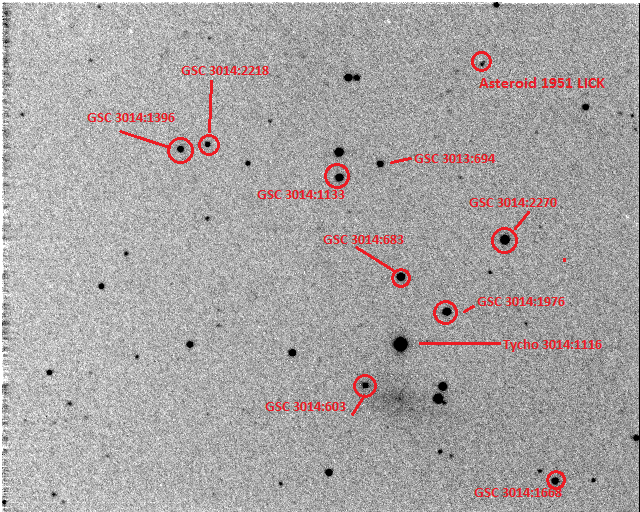
\includegraphics[width=\textwidth]{LSPR_annotated_images/Jul8Series2.png}
\end{figure}



\begin{center}
\begin{tabular}{| c |  c | c | c | c |  c | }
\hline
Star &  $x^{\text{star}}_{\text{pixel}}$ & $y^{\text{star}}_{\text{pixel}}$  & $\alpha_{\text{star}}$ &  $\delta_{\text{star}}$ \\ \hline \hline
Tycho 3014:1116 &\multicolumn{4}{|c|}{Omitted as location contains many stars} \\ \hline
GSC 3014:694 & 379.810 & 163.346 & 11h 50m 52.11 $\pm 0.0129$s & 39\degrees \space 00' 32.69$\pm 0.157$'' \\ \hline
GSC 3014:2270 & 504.524 & 239.082 & 11h 50m 32.62 $\pm 0.0117$s & 38\degrees \space 57' 38.98$\pm 0.0834$'' \\ \hline
GSC 3014:683 & 400.497 & 276.367 & 11h 50m 50.66 $\pm 0.00303$s & 38\degrees \space 56' 47.78$\pm 0.153$'' \\ \hline
GSC 3014:1976 & 446.502 & 311.219 & 11h 50m 43.57 $\pm 0.0142$s & 38\degrees \space 55' 30.58$\pm 0.0973$'' \\ \hline
GSC 3014:603 & 364.860 & 384.983 & 11h 50m 58.52 $\pm 0.00259$s & 38\degrees \space 53' 23.48$\pm 0.0477$'' \\ \hline
GSC 3014:1133 & 339.221 & 177.058 & 11h 50m 59.18 $\pm 0.0255$s & 39\degrees \space 00' 14.18$\pm 0.0203$'' \\ \hline
GSC 3014:1396 & 180.112 & 148.672 & 11h 51m 25.29 $\pm 0.00892$s & 39\degrees \space 01' 42.06$\pm 0.0267$'' \\ \hline
GSC 3014:2218 & 207.178 & 143.803 & 11h 51m 20.66 $\pm 0.00645$s & 39\degrees \space 01' 45.94$\pm 0.079$'' \\ \hline
GSC 3014:1668 & 554.745 & 480.383 & 11h 50m 28.51 $\pm 2.53\cdot 10^{-04}$s & 38\degrees \space 49' 38.31$\pm 0.0626$'' \\ \hline
UCAC3 259:110729 & 585.183 & 106.695 & 11h 50m 16.76 $\pm 0.00311$s & 39\degrees \space 01' 40.23$\pm 0.0507$'' \\ \hline
UCAC3 259:110737 & 347.984 & 76.950 & 11h 50m 55.91 $\pm 0.0158$s & 39\degrees \space 03' 27.57$\pm 0.05$'' \\ \hline
\end{tabular}
\end{center}

%%%%%%%%%%%%%%%%%%%%%%%%%%%%%%%%%%%%%%%%%%%%%%%%%%%%%%%%%%%%%%%%%%%%%%

\clearpage
\section*{July 8, 2011}
\subsection{Series 3}
\begin{center}
\begin{tabular}{| c |  c | c | c | }
\hline
JD & UT & \# images & Filter \\ \hline
2455750.738220 & 05h 43m 02.2s & 7 & Clear \\ \hline
\end{tabular}
\end{center}
\begin{center}
\begin{tabular}{| c |  c | c | c | c |  c |  c |  c | }
\hline
$x^{\text{asteroid}}_{\text{pixel}}$ & $x^{\text{asteroid}}_{\text{pixel}}$  & $\alpha_{\text{asteroid}}$ & $\delta_{\text{asteroid}}$ \\ \hline \hline
468.416  & 60.712  & 11h 50m 34.834$\pm$0.0113s & 39\degrees \space 3' 16.64$\pm$0.143'' \\ \hline 
\end{tabular}
\end{center}

\begin{figure}[h!]
  \centering
%  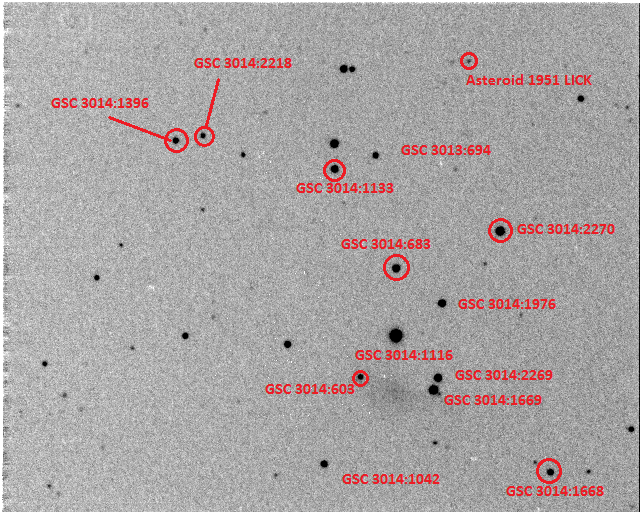
\includegraphics[width=\textwidth]{LSPR_annotated_images/Jul8Series3.png}
\end{figure}


\begin{center}
\begin{tabular}{| c |  c | c | c | c |  c | }
\hline
Star &  $x^{\text{star}}_{\text{pixel}}$ & $y^{\text{star}}_{\text{pixel}}$  & $\alpha_{\text{star}}$ &  $\delta_{\text{star}}$ \\ \hline \hline
GSC 3013:1116 &\multicolumn{4}{|c|}{Omitted as location contains many stars} \\ \hline
GSC 3014:694 & 375.136 & 154.843 & 11h 50m 52.11 $\pm 0.00127$s & 39\degrees \space 00' 32.66$\pm 0.272$'' \\ \hline
GSC 3014:2270 & 499.686 & 230.557 & 11h 50m 32.62 $\pm 0.00356$s & 38\degrees \space 57' 38.98$\pm 0.0255$'' \\ \hline
GSC 3014:683 & 395.767 & 267.828 & 11h 50m 50.66 $\pm 0.0104$s & 38\degrees \space 56' 47.78$\pm 0.053$'' \\ \hline
GSC 3014:1976 & 441.681 & 302.697 & 11h 50m 43.57 $\pm 0.0206$s & 38\degrees \space 55' 30.58$\pm 0.211$'' \\ \hline
GSC 3014:603 & 360.014 & 376.380 & 11h 50m 58.52 $\pm 0.0134$s & 38\degrees \space 53' 23.48$\pm 0.0426$'' \\ \hline
GSC 3014:1133 & 334.348 & 168.482 & 11h 50m 59.18 $\pm 0.00653$s & 39\degrees \space 00' 14.18$\pm 1.65\cdot 10^{-04}$'' \\ \hline
GSC 3014:1396 & 175.333 & 140.012 & 11h 51m 25.29 $\pm 0.00183$s & 39\degrees \space 01' 42.06$\pm 0.0987$'' \\ \hline
GSC 3014:2218 & 202.476 & 135.209 & 11h 51m 20.66 $\pm 0.001$s & 39\degrees \space 01' 45.94$\pm 0.0705$'' \\ \hline
GSC 3014:1668 & 550.000 & 471.709 & 11h 50m 28.51 $\pm 0.0141$s & 38\degrees \space 49' 38.31$\pm 0.0721$'' \\ \hline
UCAC3 259:110729 & 580.384 & 98.129 & 11h 50m 16.75 $\pm 0.00665$s & 39\degrees \space 01' 40.23$\pm 0.141$'' \\ \hline
UCAC3 259:110737 & 343.347 & 68.366 & 11h 50m 55.91 $\pm 0.00403$s & 39\degrees \space 03' 27.57$\pm 0.021$'' \\ \hline
\end{tabular}
\end{center}

%%%%%%%%%%%%%%%%%%%%%%%%%%%%%%%%%%%%%%%%%%%%%%%%%%%%%%%%%%%%%%%%%%%%%%

\clearpage
\section*{July 8, 2011}
\subsection{Series 4}
\begin{center}
\begin{tabular}{| c |  c | c | c | }
\hline
JD & UT & \# images & Filter \\ \hline
2455750.74774 & 05h 56m 44.7s & 7 & Clear \\ \hline
\end{tabular}
\end{center}
\begin{center}
\begin{tabular}{| c |  c | c | c | c |  c |  c |  c | }
\hline
$x^{\text{asteroid}}_{\text{pixel}}$ & $x^{\text{asteroid}}_{\text{pixel}}$  & $\alpha_{\text{asteroid}}$ & $\delta_{\text{asteroid}}$ \\ \hline \hline
452.115  & 63.712  & 11h 50m 36.644$\pm$0.00909s & 39\degrees \space 3' 4.32$\pm$0.170'' \\ \hline 
\end{tabular}
\end{center}

\begin{figure}[h!]
  \centering
  %  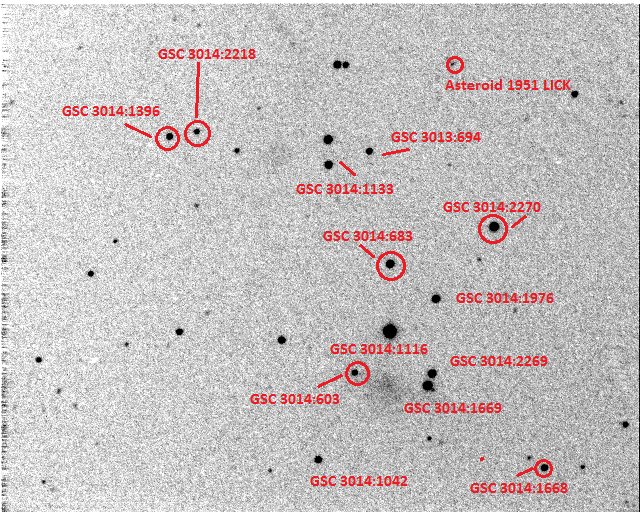
\includegraphics[width=\textwidth]{LSPR_annotated_images/Jul8Series4.png}
\end{figure}


\begin{center}
\begin{tabular}{| c |  c | c | c | c |  c | }
\hline
Star &  $x^{\text{star}}_{\text{pixel}}$ & $y^{\text{star}}_{\text{pixel}}$  & $\alpha_{\text{star}}$ &  $\delta_{\text{star}}$ \\ \hline \hline
Tycho 3014:1116 &\multicolumn{4}{|c|}{Omitted as location contains many stars} \\ \hline
GSC 3014:694 & 368.954 & 150.575 & 11h 50m 52.11 $\pm 0.00794$s & 39\degrees \space 00' 32.69$\pm 0.365$'' \\ \hline
GSC 3014:2270 & 493.660 & 226.073 & 11h 50m 32.62 $\pm 0.0113$s & 38\degrees \space 57' 38.98$\pm 0.0858$'' \\ \hline
GSC 3014:683 & 389.736 & 263.453 & 11h 50m 50.66 $\pm 0.00633$s & 38\degrees \space 56' 47.78$\pm 0.129$'' \\ \hline
GSC 3014:1976 & 435.681 & 298.265 & 11h 50m 43.58 $\pm 0.0146$s & 38\degrees \space 55' 30.56$\pm 0.108$'' \\ \hline
GSC 3014:603 & 354.254 & 372.084 & 11h 50m 58.52 $\pm 0.00444$s & 38\degrees \space 53' 23.48$\pm 0.0082$'' \\ \hline
GSC 3014:1133 & 328.216 & 164.279 & 11h 50m 59.18 $\pm 0.00119$s & 39\degrees \space 00' 14.18$\pm 0.111$'' \\ \hline
GSC 3014:1396 & 169.214 & 135.975 & 11h 51m 25.29 $\pm 0.00116$s & 39\degrees \space 01' 42.06$\pm 0.00316$'' \\ \hline
GSC 3014:2218 & 196.407 & 131.021 & 11h 51m 20.66 $\pm 0.00841$s & 39\degrees \space 01' 45.94$\pm 0.2$'' \\ \hline
GSC 3014:1668 & 544.105 & 467.212 & 11h 50m 28.51 $\pm 0.00273$s & 38\degrees \space 49' 38.31$\pm 0.0358$'' \\ \hline
UCAC3 259:110729 & 574.212 & 93.622 & 11h 50m 16.75 $\pm 0.00454$s & 39\degrees \space 01' 40.23$\pm 0.0946$'' \\ \hline
UCAC3 259:110737 & 337.036 & 64.079 & 11h 50m 55.91 $\pm 0.00986$s & 39\degrees \space 03' 27.57$\pm 0.0435$'' \\ \hline
\end{tabular}
\end{center}



%%%%%%%%%%%%%%%%%%%%%%%%%%%%%%%%%%%%%%%%%%%%%%%%%%%%%%%%%%%%%%%%%%%%%%
%%%%%%%%%%%%%%%%%%%%%%%%%%%%%%%%%    JUL 10     %%%%%%%%%%%%%%%%%%%%%%%%%%%%%

\clearpage
\section{July 10, 2011}
\subsection{Series 1}
\begin{center}
\begin{tabular}{| c |  c | c | c | }
\hline
JD & UT & \# images & Filter \\ \hline
2455752.68928 & 04h 32m 33.8s & 7 & Clear \\ \hline
\end{tabular}
\end{center}
\begin{center}
\begin{tabular}{| c |  c | c | c | c |  c |  c |  c | }
\hline
$x^{\text{asteroid}}_{\text{pixel}}$ & $x^{\text{asteroid}}_{\text{pixel}}$  & $\alpha_{\text{asteroid}}$ & $\delta_{\text{asteroid}}$ \\ \hline \hline
484.394  & 103.697  & 11h 56m 37.351$\pm$0.0154s & 38\degrees \space 23' 33.02$\pm$0.150'' \\ \hline 
\end{tabular}
\end{center}

\begin{figure}[h!]
  \centering
%   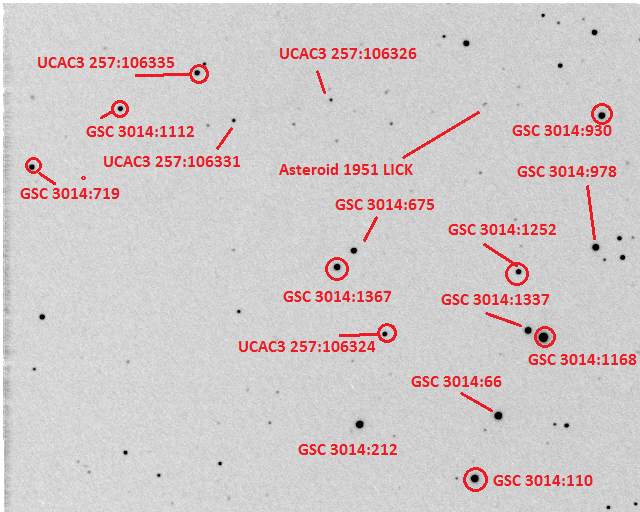
\includegraphics[width=\textwidth]{LSPR_annotated_images/Jul10Series1.png}
\end{figure}


\begin{center}
\begin{tabular}{| c |  c | c | c | c |  c | }
\hline
Star &  $x^{\text{star}}_{\text{pixel}}$ & $y^{\text{star}}_{\text{pixel}}$  & $\alpha_{\text{star}}$ &  $\delta_{\text{star}}$ \\ \hline \hline
GSC 3014:212 & 359.237 & 423.882 & 11h 57m 03.71 $\pm 0.0216$s & 38\degrees \space 13' 35.20$\pm 0.126$'' \\ \hline
GSC 3014:110 & 474.299 & 478.012 & 11h 56m 45.66 $\pm 0.00716$s & 38\degrees \space 11' 25.74$\pm 0.178$'' \\ \hline
GSC 3014:66 & 497.884 & 415.207 & 11h 56m 40.64 $\pm 0.00194$s & 38\degrees \space 13' 23.55$\pm 0.21$'' \\ \hline
GSC 3014:1168 & 542.880 & 336.847 & 11h 56m 31.81 $\pm 0.00317$s & 38\degrees \space 15' 46.65$\pm 0.095$'' \\ \hline
GSC 3014:1337 & 527.675 & 329.902 & 11h 56m 34.18 $\pm 0.02$s & 38\degrees \space 16' 03.26$\pm 0.018$'' \\ \hline
UCAC3 257:106324 & 384.331 & 333.524 & 11h 56m 57.99 $\pm 0.00221$s & 38\degrees \space 16' 26.17$\pm 0.00552$'' \\ \hline
GSC 3014:1367 & 336.679 & 266.540 & 11h 57m 04.72 $\pm 0.0132$s & 38\degrees \space 18' 46.60$\pm 0.0376$'' \\ \hline
GSC 3014:675 & 353.358 & 250.105 & 11h 57m 01.67 $\pm 0.0147$s & 38\degrees \space 19' 15.00$\pm 0.125$'' \\ \hline
GSC 3014:1252 & 518.140 & 271.224 & 11h 56m 34.73 $\pm 0.00634$s & 38\degrees \space 17' 59.62$\pm 0.0308$'' \\ \hline
GSC 3014:978 & 595.301 & 246.811 & 11h 56m 21.56 $\pm 0.036$s & 38\degrees \space 18' 31.00$\pm 0.0936$'' \\ \hline
GSC 3014:930 & 601.337 & 115.069 & 11h 56m 18.16 $\pm 0.00777$s & 38\degrees \space 22' 46.24$\pm 0.017$'' \\ \hline
UCAC3 257:106331 & 233.281 & 119.964 & 11h 57m 19.28 $\pm 1.44\cdot 10^{-04}$s & 38\degrees \space 23' 53.27$\pm 0.25$'' \\ \hline
GSC 3014:1112 & 119.942 & 108.070 & 11h 57m 37.88 $\pm 0.007$s & 38\degrees \space 24' 40.02$\pm 0.0712$'' \\ \hline
UCAC3 257:106335 & 196.700 & 72.257 & 11h 57m 24.50 $\pm 0.0162$s & 38\degrees \space 25' 34.04$\pm 0.0351$'' \\ \hline
GSC 3014:719 & 31.421 & 166.583 & 11h 57m 53.57 $\pm 0.00414$s & 38\degrees \space 23' 04.15$\pm 0.201$'' \\ \hline
GSC 3014:1338 & 465.809 & 42.768 & 11h 56m 39.36 $\pm 0.00827$s & 38\degrees \space 25' 35.36$\pm 0.259$'' \\ \hline
GSC 3014:1291 & 559.792 & 65.079 & 11h 56m 24.14 $\pm 0.0215$s & 38\degrees \space 24' 32.59$\pm 0.185$'' \\ \hline
GSC 3014:1303 & 594.049 & 31.890 & 11h 56m 17.89 $\pm 0.00381$s & 38\degrees \space 25' 29.83$\pm 0.00699$'' \\ \hline
\end{tabular}
\end{center}

%%%%%%%%%%%%%%%%%%%%%%%%%%%%%%%%%%%%%%%%%%%%%%%%%%%%%%%%%%%%%%%%%%%%%%

\clearpage
\section*{July 10, 2011}
\subsection{Series 2}
\begin{center}
\begin{tabular}{| c |  c | c | c | }
\hline
JD & UT & \# images & Filter \\ \hline
2455752.70592 & 04h 56m 31.5s & 7 & Clear \\ \hline
\end{tabular}
\end{center}
\begin{center}
\begin{tabular}{| c |  c | c | c | c |  c |  c |  c | }
\hline
$x^{\text{asteroid}}_{\text{pixel}}$ & $x^{\text{asteroid}}_{\text{pixel}}$  & $\alpha_{\text{asteroid}}$ & $\delta_{\text{asteroid}}$ \\ \hline \hline
499.065  & 68.756  & 11h 56m 40.336$\pm$0.0113s & 38\degrees \space 23' 13.08$\pm$0.0921'' \\ \hline 
\end{tabular}
\end{center}

\begin{figure}[h!]
  \centering
 % 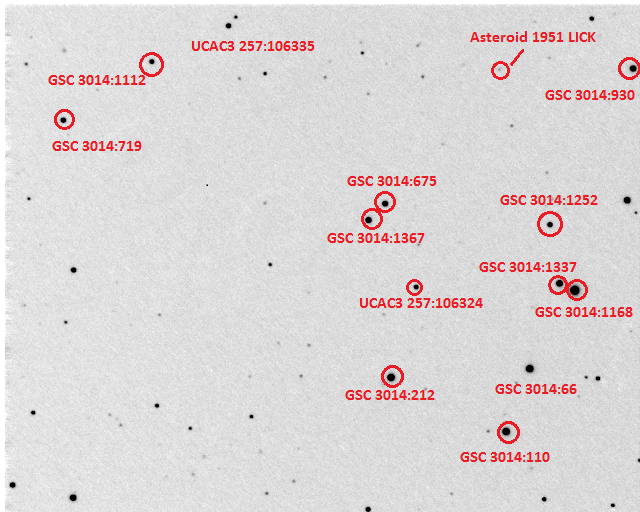
\includegraphics[width=\textwidth]{LSPR_annotated_images/Jul10Series2.png}
\end{figure}


\begin{center}
\begin{tabular}{| c |  c | c | c | c |  c | }
\hline
Star &  $x^{\text{star}}_{\text{pixel}}$ & $y^{\text{star}}_{\text{pixel}}$  & $\alpha_{\text{star}}$ &  $\delta_{\text{star}}$ \\ \hline \hline
GSC 3014:212 & 390.715 & 376.826 & 11h 57m 03.71 $\pm 0.0133$s & 38\degrees \space 13' 35.20$\pm 0.13$'' \\ \hline
GSC 3014:110 & 505.688 & 431.017 & 11h 56m 45.66 $\pm 0.00423$s & 38\degrees \space 11' 25.74$\pm 0.016$'' \\ \hline
GSC 3014:66 &\multicolumn{4}{|c|}{Omitted due stong database disagreement} \\ \hline
GSC 3014:1168 & 574.317 & 289.795 & 11h 56m 31.81 $\pm 0.0142$s & 38\degrees \space 15' 46.65$\pm 0.139$'' \\ \hline
GSC 3014:1337 & 559.084 & 282.854 & 11h 56m 34.18 $\pm 0.0143$s & 38\degrees \space 16' 03.26$\pm 0.0151$'' \\ \hline
UCAC3 257:106324 & 415.754 & 286.521 & 11h 56m 57.99 $\pm 0.00158$s & 38\degrees \space 16' 26.17$\pm 0.0511$'' \\ \hline
GSC 3014:1367 & 368.110 & 219.550 & 11h 57m 04.72 $\pm 0.0137$s & 38\degrees \space 18' 46.60$\pm 0.0421$'' \\ \hline
GSC 3014:675 & 384.769 & 203.108 & 11h 57m 01.67 $\pm 0.0129$s & 38\degrees \space 19' 15.00$\pm 0.139$'' \\ \hline
GSC 3014:1252 & 549.518 & 224.160 & 11h 56m 34.73 $\pm 0.00509$s & 38\degrees \space 17' 59.62$\pm 0.0154$'' \\ \hline
GSC 3014:978 &\multicolumn{4}{|c|}{Omitted due stong database disagreement} \\ \hline
GSC 3014:930 & 632.693 & 68.047 & 11h 56m 18.16 $\pm 0.00494$s & 38\degrees \space 22' 46.24$\pm 0.0351$'' \\ \hline
UCAC3 257:106326 &\multicolumn{4}{|c|}{Omitted due stong database disagreement} \\ \hline
UCAC3 257:106331 &\multicolumn{4}{|c|}{Omitted due stong database disagreement} \\ \hline
GSC 3014:1112 & 151.369 & 61.144 & 11h 57m 37.88 $\pm 0.00202$s & 38\degrees \space 24' 40.02$\pm 0.019$'' \\ \hline
UCAC3 257:106335 &\multicolumn{4}{|c|}{Omitted due stong database disagreement} \\ \hline
GSC 3014:719 & 62.882 & 119.642 & 11h 57m 53.57 $\pm 0.00379$s & 38\degrees \space 23' 04.15$\pm 0.0754$'' \\ \hline
\end{tabular}
\end{center}

%%%%%%%%%%%%%%%%%%%%%%%%%%%%%%%%%%%%%%%%%%%%%%%%%%%%%%%%%%%%%%%%%%%%%%

\clearpage
\section*{July 10, 2011}
\subsection{Series 3}
\begin{center}
\begin{tabular}{| c |  c | c | c | }
\hline
JD & UT & \# images & Filter \\ \hline
2455752.71975 & 05h 16m 26.4s & 7 & Clear \\ \hline
\end{tabular}
\end{center}
\begin{center}
\begin{tabular}{| c |  c | c | c | c |  c |  c |  c | }
\hline
$x^{\text{asteroid}}_{\text{pixel}}$ & $x^{\text{asteroid}}_{\text{pixel}}$  & $\alpha_{\text{asteroid}}$ & $\delta_{\text{asteroid}}$ \\ \hline \hline
474.601  & 60.254  & 11h 56m 42.870$\pm$0.0104s & 38\degrees \space 22' 52.39$\pm$0.0682'' \\ \hline 
\end{tabular}
\end{center}

\begin{figure}[h!]
  \centering
  %  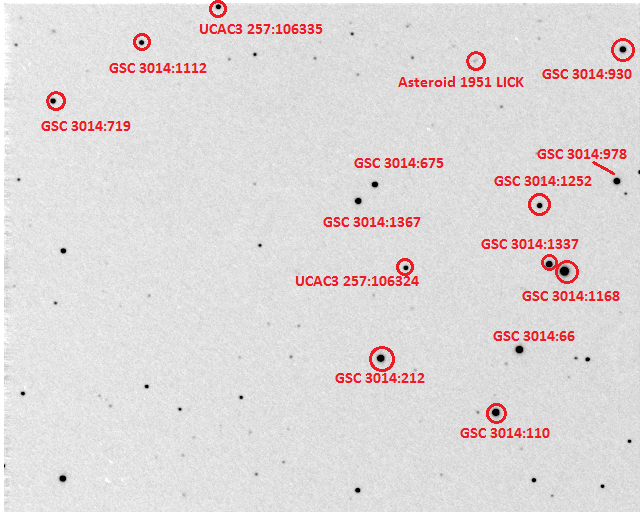
\includegraphics[width=0.75\textwidth]{LSPR_annotated_images/Jul10Series3.png}
\end{figure}


\begin{center}
\begin{tabular}{| c |  c | c | c | c |  c | }
\hline
Star &  $x^{\text{star}}_{\text{pixel}}$ & $y^{\text{star}}_{\text{pixel}}$  & $\alpha_{\text{star}}$ &  $\delta_{\text{star}}$ \\ \hline \hline
GSC 3014:212 & 380.384 & 357.718 & 11h 57m 03.71$\pm 0.0131$s & 38\degrees \space 13' 35.20$\pm 0.0827$'' \\ \hline
GSC 3014:110 & 495.385 & 411.898 & 11h 56m 45.66$\pm 0.0108$s & 38\degrees \space 11' 25.74$\pm 0.0446$'' \\ \hline
GSC 3014:66 &\multicolumn{4}{|c|}{Omitted to improve fit} \\ \hline
GSC 3014:1168 & 563.978 & 270.678 & 11h 56m 31.81$\pm 0.0137$s & 38\degrees \space 15' 46.65$\pm 0.13$'' \\ \hline
GSC 3014:1337 & 548.742 & 263.706 & 11h 56m 34.18$\pm 0.0149$s & 38\degrees \space 16' 03.26$\pm 0.0549$'' \\ \hline
UCAC 257:106324 & 405.454 & 267.347 & 11h 56m 57.99$\pm 0.00414$s & 38\degrees \space 16' 26.17$\pm 0.0432$'' \\ \hline
GSC 3014:1367 &\multicolumn{4}{|c|}{Omitted to improve fit} \\ \hline
GSC 3014:675 &\multicolumn{4}{|c|}{Omitted to improve fit} \\ \hline
GSC 3014:1252 & 539.194 & 205.059 & 11h 56m 34.73$\pm 0.00433$s & 38\degrees \space 17' 59.62$\pm 2.76\cdot 10^{-4}$'' \\ \hline
GSC 3014:978 &\multicolumn{4}{|c|}{Omitted to improve fit} \\ \hline
GSC 3014:930 & 622.407 & 48.957 & 11h 56m 18.16$\pm 8.15\cdot 10^{-4}$s & 38\degrees \space 22' 46.24$\pm 0.0286$'' \\ \hline
UCAC3 257:106326 &\multicolumn{4}{|c|}{Omitted to improve fit} \\ \hline
UCAC3 257:106331 &\multicolumn{4}{|c|}{Omitted to improve fit} \\ \hline
GSC 3014:1112 & 141.113 & 42.039 & 11h 57m 37.88$\pm 0.00538$s & 38\degrees \space 24' 40.02$\pm 0.0203$'' \\ \hline
UCAC3 257:106335 & 217.938 & 6.218 & 11h 57m 24.50$\pm 0.00239$s & 38\degrees \space 25' 34.04$\pm 0.0125$'' \\ \hline
GSC 3014:719 & 52.598 & 100.484 & 11h 57m 53.57$\pm 9.67$s & 38\degrees \space 23' 04.15$\pm 0.027$'' \\ \hline
\end{tabular}
\end{center}

%%%%%%%%%%%%%%%%%%%%%%%%%%%%%%%%%%%%%%%%%%%%%%%%%%%%%%%%%%%%%%%%%%%%%%
%%%%%%%%%%%%%%%%%%%%%%%%%%%%%%%%%    JUL 16     %%%%%%%%%%%%%%%%%%%%%%%%%%%%%



\clearpage
\section{July 16, 2011}
\subsection{Series 1}
\begin{center}
\begin{tabular}{| c |  c | c | c | }
\hline
JD & UT & \# images & Filter \\ \hline
2455758.69142 & 04h 35m 38.5s & 5 & V-Filter \\ \hline
\end{tabular}
\end{center}

\begin{figure}[h!]
  \centering
  % 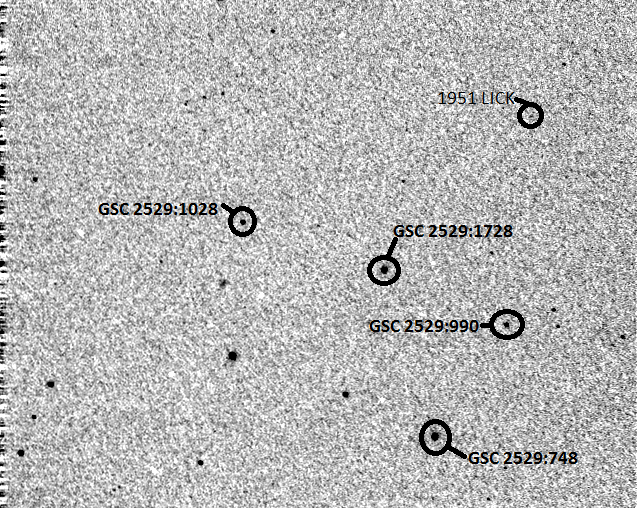
\includegraphics[width=\textwidth]{LSPR_annotated_images/Jul16Series1.png}
\end{figure}

Asteroid apparent magnitude $\approx$ 16.62

Image is very noisy, asteroid is impossible to detect without assistance from other series. Another V-filter image should be taken.

\begin{center}
\begin{tabular}{| c |  c | c | c | c |  c | }
\hline
Star & NOMAD Apparent Magnitude & Measured Apparent Magnitude \\ \hline \hline
GSC 2529:1028 & 13.86 & Used for calibration \\ \hline
GSC 2529:1728 & 12.52 & 12.39 \\ \hline
GSC 2529:990 & 15.53 & 14.06 \\ \hline
GSC 2529:748 & 11.95 & 11.71 \\ \hline
\end{tabular}
\end{center}

%%%%%%%%%%%%%%%%%%%%%%%%%%%%%%%%%%%%%%%%%%%%%%%%%%%%%%%%%%%%%%%%%%%%%%


\clearpage
\section*{July 16, 2011}
\subsection{Series 2}
\begin{center}
\begin{tabular}{| c |  c | c | c | }
\hline
JD & UT & \# images & Filter \\ \hline
2455758.69609 & 04h 42m 22.2s & 5 & Clear \\ \hline
\end{tabular}
\end{center}
\begin{center}
\begin{tabular}{| c |  c | c | c | c |  c |  c |  c | }
\hline
$x^{\text{asteroid}}_{\text{pixel}}$ & $x^{\text{asteroid}}_{\text{pixel}}$  & $\alpha_{\text{asteroid}}$ & $\delta_{\text{asteroid}}$ \\ \hline \hline
525.040  & 118.082  & 12h 15m 3.471$\pm$0.0193s & 36\degrees \space 13' 55.36$\pm$0.185'' \\ \hline 
\end{tabular}
\end{center}

\begin{figure}[h!]
  \centering
  % 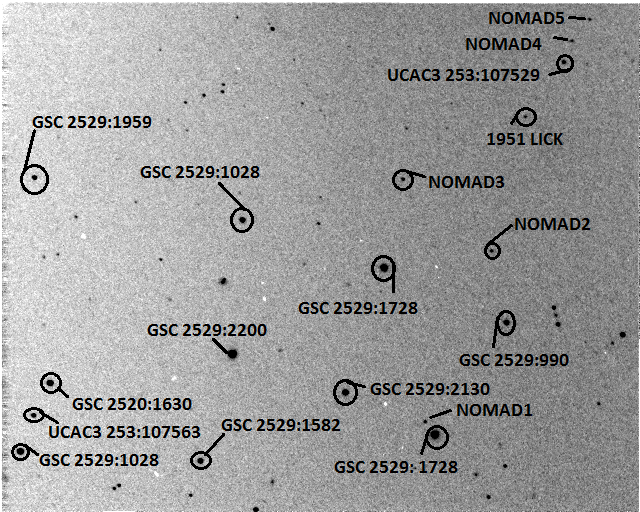
\includegraphics[width=\textwidth]{LSPR_annotated_images/Jul16Series2.png}
\end{figure}

Image clear and well focused. Many well-measured stars in starfield. In this sense very confident about this observation. However, asteroid is located far from center, and not really surrounded by reference stars.

\begin{center}
\begin{tabular}{| c |  c | c | c | c |  c | }
\hline
Star &  $x^{\text{star}}_{\text{pixel}}$ & $y^{\text{star}}_{\text{pixel}}$  & $\alpha_{\text{star}}$ &  $\delta_{\text{star}}$ \\ \hline \hline
GSC 2529:1028 & 242.235 & 219.541 & 12h 15m 46.86 $\pm 0.00787$s & 36\degrees \space 9' 28.87$\pm 0.0929$'' \\ \hline
GSC 2529:1728 & 383.760 & 267.365 & 12h 15m 23.25 $\pm 0.011$s & 36\degrees \space 8' 28.92$\pm 0.0519$'' \\ \hline
GSC 2529:990 & 506.192 & 322.147 & 12h 15m 2.53 $\pm 0.0216$s & 36\degrees \space 7' 10.46$\pm 0.123$'' \\ \hline
GSC 2529:748 & 434.534 & 433.966 & 12h 15m 11.94 $\pm 0.0213$s & 36\degrees \space 3' 16.62$\pm 0.164$'' \\ \hline
GSC 2529:2130 & 345.107 & 391.969 & 12h 15m 27.04 $\pm 0.0154$s & 36\degrees \space 4' 17.84$\pm 0.072$'' \\ \hline
GSC 2529:2200 &\multicolumn{4}{|c|}{Omitted as it is a double star} \\ \hline
NOMAD1 &\multicolumn{4}{|c|}{Omitted due to bad image quality} \\ \hline
GSC 2529:1582 & 200.099 & 460.414 & 12h 15m 48.97 $\pm 0.0105$s & 36\degrees \space 1' 31.18$\pm 0.111$'' \\ \hline
GSC 2529:1630 & 49.937 & 382.487 & 12h 16m 14.55 $\pm 8.15\cdot 10^{-04}$s & 36\degrees \space 3' 27.25$\pm 0.0552$'' \\ \hline
UCAC3 253:107563 & 33.452 & 414.901 & 12h 16m 16.58 $\pm 0.0201$s & 36\degrees \space 2' 20.50$\pm 0.0546$'' \\ \hline
GSC 2529:1048 & 20.259 & 450.861 & 12h 16m 17.96 $\pm 0.0133$s & 36\degrees \space 1' 7.53$\pm 0.0601$'' \\ \hline
NOMAD2 & 491.172 & 250.237 & 12h 15m 06.34 $\pm 0.0126$s & 36\degrees \space 9' 26.92$\pm 0.0169$'' \\ \hline
NOMAD3 & 402.706 & 178.513 & 12h 15m 21.91 $\pm 0.0131$s & 36\degrees \space 11' 26.05$\pm 0.123$'' \\ \hline
UCAC3 253:107529 & 563.464 & 61.580 & 12h 14m 58.29 $\pm 0.00908$s & 36\degrees \space 15' 50.23$\pm 0.0617$'' \\ \hline
GSC 2529:1959 & 34.287 & 177.111 & 12h 16m 21.06 $\pm 0.00122$s & 36\degrees \space 10' 02.53$\pm 0.116$'' \\ \hline
NOMAD4 &\multicolumn{4}{|c|}{Omitted due to bad image quality} \\ \hline
NOMAD5 &\multicolumn{4}{|c|}{Omitted due to bad image quality} \\ \hline
\end{tabular}
\end{center}

%%%%%%%%%%%%%%%%%%%%%%%%%%%%%%%%%%%%%%%%%%%%%%%%%%%%%%%%%%%%%%%%%%%%%%

\clearpage
\section*{July 16, 2011}
\subsection{Series 3}
\begin{center}
\begin{tabular}{| c |  c | c | c | }
\hline
JD & UT & \# images & Filter \\ \hline
2455758.70920 & 05h 01m 14.9s & 5 & Clear \\ \hline
\end{tabular}
\end{center}
\begin{center}
\begin{tabular}{| c |  c | c | c | c |  c |  c |  c | }
\hline
$x^{\text{asteroid}}_{\text{pixel}}$ & $x^{\text{asteroid}}_{\text{pixel}}$  & $\alpha_{\text{asteroid}}$ & $\delta_{\text{asteroid}}$ \\ \hline \hline
509.873 & 90.518 & 12h 15m 5.936$\pm$0.0259s & 36\degrees \space 13' 37.40$\pm$0.125'' \\ \hline 
\end{tabular}
\end{center}

\begin{figure}[h!]
  \centering
   %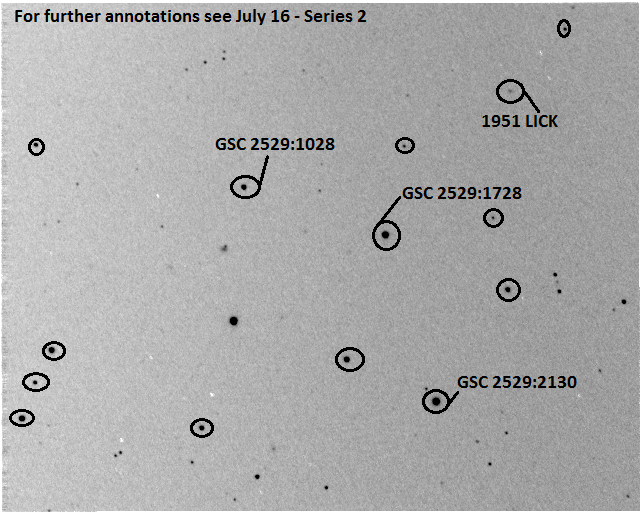
\includegraphics[width=\textwidth]{LSPR_annotated_images/Jul16Series3.png}
\end{figure}

\begin{center}
\begin{tabular}{| c |  c | c | c | c |  c | }
\hline
Star &  $x^{\text{star}}_{\text{pixel}}$ & $y^{\text{star}}_{\text{pixel}}$  & $\alpha_{\text{star}}$ &  $\delta_{\text{star}}$ \\ \hline \hline
GSC 2529:1028 & 243.438 & 186.648 & 12h 15m 46.86 $\pm 0.0142$s & 36\degrees \space 9' 28.87$\pm 0.0999$'' \\ \hline
GSC 2529:1728 & 384.947 & 234.420 & 12h 15m 23.25 $\pm 7.09\cdot 10^{-04}$s & 36\degrees \space 8' 28.92$\pm 0.00879$'' \\ \hline
GSC 2529:990 & 507.400 & 289.204 & 12h 15m 2.53 $\pm 0.0317$s & 36\degrees \space 7' 10.46$\pm 0.142$'' \\ \hline
GSC 2529:748 & 435.783 & 401.019 & 12h 15m 11.94 $\pm 0.0169$s & 36\degrees \space 3' 16.62$\pm 0.184$'' \\ \hline
GSC 2529:2130 & 346.312 & 359.031 & 12h 15m 27.04 $\pm 0.0255$s & 36\degrees \space 4' 17.84$\pm 0.0494$'' \\ \hline
GSC 2529:2200 &\multicolumn{4}{|c|}{Omitted as it is a double star} \\ \hline
NOMAD1 &\multicolumn{4}{|c|}{Omitted due to bad image quality} \\ \hline
GSC 2529:1582 & 201.324 & 427.459 & 12h 15m 48.97 $\pm 0.0172$s & 36\degrees \space 1' 31.18$\pm 0.0405$'' \\ \hline
GSC 2529:1630 & 51.251 & 349.620 & 12h 16m 14.55 $\pm 0.0124$s & 36\degrees \space 3' 27.25$\pm 0.0303$'' \\ \hline
UCAC3 253:107563 & 34.653 & 382.035 & 12h 16m 16.58 $\pm 0.0133$s & 36\degrees \space 2' 20.50$\pm 0.114$'' \\ \hline
GSC 2529:1048 & 21.570 & 417.978 & 12h 16m 17.96 $\pm 0.00323$s & 36\degrees \space 1' 7.53$\pm 0.0686$'' \\ \hline
NOMAD2 & 492.684 & 217.441 & 12h 15m 06.34 $\pm 0.0551$s & 36\degrees \space 9' 26.92$\pm 0.189$'' \\ \hline
NOMAD3 & 404.004 & 145.622 & 12h 15m 21.91 $\pm 0.0212$s & 36\degrees \space 11' 26.05$\pm 0.12$'' \\ \hline
UCAC3 253:107529 & 564.641 & 28.658 & 12h 14m 58.29 $\pm 0.0209$s & 36\degrees \space 15' 50.23$\pm 0.0255$'' \\ \hline
GSC 2529:1959 & 35.486 & 144.237 & 12h 16m 21.06 $\pm 0.00541$s & 36\degrees \space 10' 02.53$\pm 0.142$'' \\ \hline
\end{tabular}
\end{center}

%%%%%%%%%%%%%%%%%%%%%%%%%%%%%%%%%%%%%%%%%%%%%%%%%%%%%%%%%%%%%%%%%%%%%%

\clearpage
\section*{July 16, 2011}
\subsection{Series 4}
\begin{center}
\begin{tabular}{| c |  c | c | c | }
\hline
JD & UT & \# images & Filter \\ \hline
2455758.71939 & 05h 15m 55.3s & 5 & Clear \\ \hline
\end{tabular}
\end{center}
\begin{center}
\begin{tabular}{| c |  c | c | c | c |  c |  c |  c | }
\hline
$x^{\text{asteroid}}_{\text{pixel}}$ & $x^{\text{asteroid}}_{\text{pixel}}$  & $\alpha_{\text{asteroid}}$ & $\delta_{\text{asteroid}}$ \\ \hline \hline
494.057& 86.436 & 12h 15m 7.671$\pm$0.0153s & 36\degrees \space 13' 22.93$\pm$0.117'' \\ \hline 
\end{tabular}
\end{center}

\begin{figure}[h!]
  \centering
   %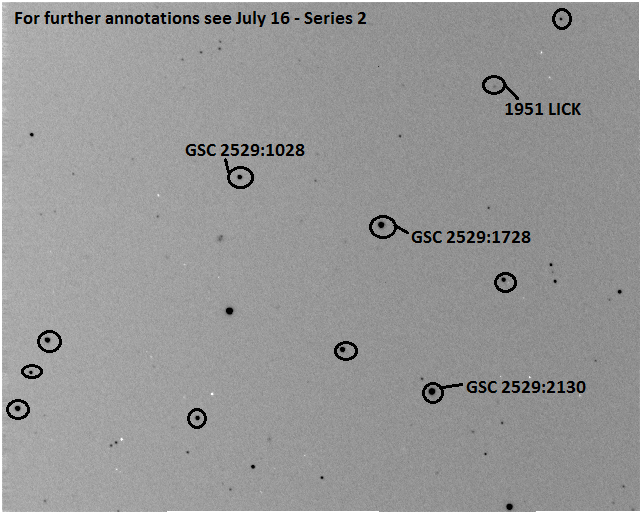
\includegraphics[width=\textwidth]{LSPR_annotated_images/Jul16Series4.png}
\end{figure}


\begin{center}
\begin{tabular}{| c |  c | c | c | c |  c | }
\hline
Star &  $x^{\text{star}}_{\text{pixel}}$ & $y^{\text{star}}_{\text{pixel}}$  & $\alpha_{\text{star}}$ &  $\delta_{\text{star}}$ \\ \hline \hline
GSC 2529:1028 & 239.229 & 176.557 & 12h 15m 46.86 $\pm 0.00736$s & 36\degrees \space 9' 28.87$\pm 0.0748$'' \\ \hline
GSC 2529:1728 & 380.704 & 224.411 & 12h 15m 23.25 $\pm 0.012$s & 36\degrees \space 8' 28.92$\pm 0.169$'' \\ \hline
GSC 2529:990 & 503.125 & 279.174 & 12h 15m 2.53 $\pm 0.0154$s & 36\degrees \space 7' 10.46$\pm 0.0207$'' \\ \hline
GSC 2529:748 & 431.437 & 390.970 & 12h 15m 11.94 $\pm 0.0234$s & 36\degrees \space 3' 16.62$\pm 0.172$'' \\ \hline
GSC 2529:2130 & 342.032 & 349.014 & 12h 15m 27.04 $\pm 0.0145$s & 36\degrees \space 4' 17.84$\pm 0.125$'' \\ \hline
GSC 2529:2200 &\multicolumn{4}{|c|}{Omitted as it is a double star} \\ \hline
NOMAD1 &\multicolumn{4}{|c|}{Omitted due to bad image quality} \\ \hline
GSC 2529:1582 & 197.026 & 417.468 & 12h 15m 48.97 $\pm 0.0127$s & 36\degrees \space 1' 31.18$\pm 0.103$'' \\ \hline
GSC 2529:1630 & 46.963 & 339.529 & 12h 16m 14.55 $\pm 0.00485$s & 36\degrees \space 3' 27.25$\pm 0.129$'' \\ \hline
UCAC3 253:107563 & 30.442 & 371.970 & 12h 16m 16.58 $\pm 0.0194$s & 36\degrees \space 2' 20.50$\pm 0.022$'' \\ \hline
GSC 2529:1048 & 17.263 & 407.921 & 12h 16m 17.96 $\pm 0.0112$s & 36\degrees \space 1' 7.53$\pm 0.0129$'' \\ \hline
NOMAD2 &\multicolumn{4}{|c|}{Omitted due to bad image quality} \\ \hline
NOMAD3 &\multicolumn{4}{|c|}{Omitted due to bad image quality} \\ \hline
UCAC3 253:107529 & 560.500 & 18.450 & 12h 14m 58.29 $\pm 0.00318$s & 36\degrees \space 15' 50.23$\pm 0.0353$'' \\ \hline
GSC 2529:1959 & 31.329 & 134.225 & 12h 16m 21.06 $\pm 0.0016$s & 36\degrees \space 10' 02.53$\pm 0.0269$'' \\ \hline
\end{tabular}
\end{center}

%%%%%%%%%%%%%%%%%%%%%%%%%%%%%%%%%%%%%%%%%%%%%%%%%%%%%%%%%%%%%%%%%%%%%%

\clearpage
\section*{July 16, 2011}
\subsection{Series 5}
\begin{center}
\begin{tabular}{| c |  c | c | c | }
\hline
JD & UT & \# images & Filter \\ \hline
2455758.72524 & 05h 24m 20.7s & 5 & Clear \\ \hline
\end{tabular}
\end{center}
\begin{center}
\begin{tabular}{| c |  c | c | c | c |  c |  c |  c | }
\hline
$x^{\text{asteroid}}_{\text{pixel}}$ & $x^{\text{asteroid}}_{\text{pixel}}$  & $\alpha_{\text{asteroid}}$ & $\delta_{\text{asteroid}}$ \\ \hline \hline
507.065 & 75.024 & 12h 15m 8.724$\pm$0.0253s & 36\degrees \space 13' 15.39$\pm$0.0949'' \\ \hline 
\end{tabular}
\end{center}

\begin{figure}[h!]
  \centering
   %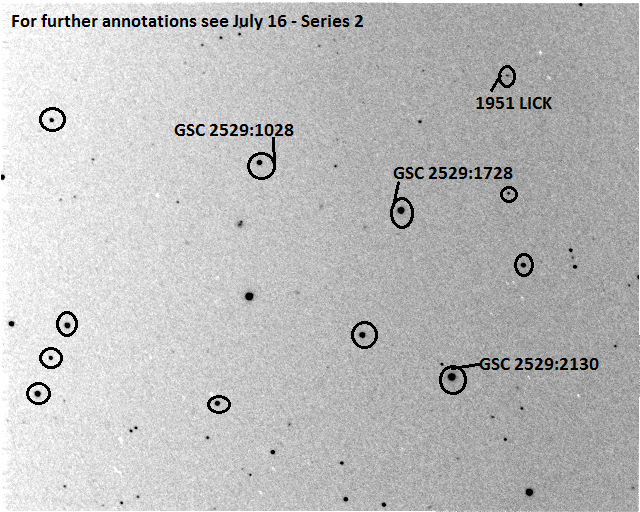
\includegraphics[width=\textwidth]{LSPR_annotated_images/Jul16Series5.png}
\end{figure}


\begin{center}
\begin{tabular}{| c |  c | c | c | c |  c | }
\hline
Star &  $x^{\text{star}}_{\text{pixel}}$ & $y^{\text{star}}_{\text{pixel}}$  & $\alpha_{\text{star}}$ &  $\delta_{\text{star}}$ \\ \hline \hline
GSC 2529:1028 & 259.045 & 162.036 & 12h 15m 46.86 $\pm 0.0231$s & 36\degrees \space 9' 28.87$\pm 0.0499$'' \\ \hline
GSC 2529:1728 & 400.540 & 209.846 & 12h 15m 23.25 $\pm 0.00231$s & 36\degrees \space 8' 28.92$\pm 0.105$'' \\ \hline
GSC 2529:990 & 522.963 & 264.629 & 12h 15m 2.53 $\pm 0.0297$s & 36\degrees \space 7' 10.46$\pm 0.0365$'' \\ \hline
GSC 2529:748 & 451.340 & 376.406 & 12h 15m 11.94 $\pm 0.0208$s & 36\degrees \space 3' 16.62$\pm 0.166$'' \\ \hline
GSC 2529:2130 & 361.898 & 334.440 & 12h 15m 27.04 $\pm 0.0227$s & 36\degrees \space 4' 17.84$\pm 0.113$'' \\ \hline
GSC 2529:2200 &\multicolumn{4}{|c|}{Omitted as it is a double star} \\ \hline
NOMAD1 &\multicolumn{4}{|c|}{Omitted due to bad image quality} \\ \hline
GSC 2529:1582 & 216.913 & 402.833 & 12h 15m 48.97 $\pm 0.0167$s & 36\degrees \space 1' 31.18$\pm 0.0286$'' \\ \hline
GSC 2529:1630 & 66.909 & 324.970 & 12h 16m 14.55 $\pm 0.0125$s & 36\degrees \space 3' 27.25$\pm 0.0867$'' \\ \hline
UCAC3 253:107563 & 50.321 & 357.367 & 12h 16m 16.58 $\pm 0.0159$s & 36\degrees \space 2' 20.50$\pm 0.0156$'' \\ \hline
GSC 2529:1048 & 37.228 & 393.363 & 12h 16m 17.96 $\pm 3.55\cdot 10^{-04}$s & 36\degrees \space 1' 7.53$\pm 0.0699$'' \\ \hline
NOMAD2 & 508.224 & 192.728 & 12h 15m 06.34 $\pm 0.0459$s & 36\degrees \space 9' 26.92$\pm 0.0442$'' \\ \hline
NOMAD3 &\multicolumn{4}{|c|}{Omitted due to bad image quality} \\ \hline
GSC 2529:1959 & 51.243 & 119.664 & 12h 16m 21.06 $\pm 7.77\cdot 10^{-04}$s & 36\degrees \space 10' 02.53$\pm 0.0368$'' \\ \hline
\end{tabular}
\end{center}

%%%%%%%%%%%%%%%%%%%%%%%%%%%%%%%%%%%%%%%%%%%%%%%%%%%%%%%%%%%%%%%%%%%%%%
%%%%%%%%%%%%%%%%%%%%%%%%%%%%%%%%%    JUL 19     %%%%%%%%%%%%%%%%%%%%%%%%%%%%%

\clearpage
\section{July 19, 2011}
\subsection{Series 1}
\begin{center}
\begin{tabular}{| c |  c | c | c | }
\hline
JD & UT & \# images & Filter \\ \hline
2455761.67894 & 04h 17m 30.4s & 7 & Clear \\ \hline
\end{tabular}
\end{center}
\begin{center}
\begin{tabular}{| c |  c | c | c | c |  c |  c |  c | }
\hline
$x^{\text{asteroid}}_{\text{pixel}}$ & $x^{\text{asteroid}}_{\text{pixel}}$  & $\alpha_{\text{asteroid}}$ & $\delta_{\text{asteroid}}$ \\ \hline \hline
526.448 &140.462 & 12h 24m 7.855$\pm$0.0157s & 35\degrees \space 5' 27.33$\pm$0.190'' \\ \hline 
\end{tabular}
\end{center}

\begin{figure}[h!]
  \centering
   %\includegraphics[width=\textwidth]{LSPR_annotated_images/Jul19Series1.png}
\end{figure}

\begin{center}
\begin{tabular}{| c |  c | c | c | c |  c | }
\hline
Star &  $x^{\text{star}}_{\text{pixel}}$ & $y^{\text{star}}_{\text{pixel}}$  & $\alpha_{\text{star}}$ &  $\delta_{\text{star}}$ \\ \hline \hline
GSC 2530:1398 & 24.520 & 88.803 & 12h 25m 28.42 $\pm 0.00168$s & 35\degrees \space 05' 11.71$\pm 0.11$'' \\ \hline
GSC 2530:1102 & 17.583 & 180.220 & 12h 25m 27.78 $\pm 0.00377$s & 35\degrees \space 02' 12.67$\pm 0.333$'' \\ \hline
GSC 2530:796 & 13.677 & 282.832 & 12h 25m 26.45 $\pm 0.0117$s & 34\degrees \space 58' 51.62$\pm 0.162$'' \\ \hline
GSC 2530:506 & 197.965 & 256.969 & 12h 24m 57.73 $\pm 0.0125$s & 35\degrees \space 00' 25.14$\pm 0.0726$'' \\ \hline
GSC 2530:1499 & 195.939 & 314.936 & 12h 24m 56.96 $\pm 0.00967$s & 34\degrees \space 58' 31.75$\pm 0.0513$'' \\ \hline
GSC 2530:1414 & 289.027 & 424.047 & 12h 24m 40.18 $\pm 0.00208$s & 34\degrees \space 55' 20.94$\pm 0.0602$'' \\ \hline
GSC 2530:1374 &\multicolumn{4}{|c|}{Omitted as it is a double star} \\ \hline
GSC 2530:1123 & 416.375 & 436.343 & 12h 24m 19.83 $\pm 0.0328$s & 34\degrees \space 55' 26.53$\pm 0.206$'' \\ \hline
GSC 2530:851 & 472.305 & 445.652 & 12h 24m 10.75 $\pm 0.0217$s & 34\degrees \space 55' 20.91$\pm 0.0776$'' \\ \hline
GSC 2530:706 & 346.750 & 158.718 & 12h 24m 36.00 $\pm 0.0113$s & 35\degrees \space 04' 10.40$\pm 0.242$'' \\ \hline
NOMAD1 & 475.801 & 99.279 & 12h 24m 16.65 $\pm 0.00522$s & 35\degrees \space 06' 35.98$\pm 0.0546$'' \\ \hline
NOMAD2 & 481.772 & 78.646 & 12h 24m 16.10 $\pm 0.00778$s & 35\degrees \space 07' 17.30$\pm 0.147$'' \\ \hline
NOMAD3 &  499.376 & 43.031 & 12h 24m 13.97 $\pm 0.00808$s & 35\degrees \space 08' 30.97$\pm 0.184$'' \\ \hline
\end{tabular}
\end{center}

%%%%%%%%%%%%%%%%%%%%%%%%%%%%%%%%%%%%%%%%%%%%%%%%%%%%%%%%%%%%%%%%%%%%%%

\clearpage
\section*{July 19, 2011}
\subsection{Series 2}
\begin{center}
\begin{tabular}{| c |  c | c | c | }
\hline
JD & UT & \# images & Filter \\ \hline
2455761.69413 & 04h 39m 32.8s & 7 & Clear \\ \hline
\end{tabular}
\end{center}
\begin{center}
\begin{tabular}{| c |  c | c | c | c |  c |  c |  c | }
\hline
$x^{\text{asteroid}}_{\text{pixel}}$ & $x^{\text{asteroid}}_{\text{pixel}}$  & $\alpha_{\text{asteroid}}$ & $\delta_{\text{asteroid}}$ \\ \hline \hline
424.151&117.621 & 12h 24m 10.630$\pm$0.0207s & 35\degrees \space 5' 5.40$\pm$0.180'' \\ \hline 
\end{tabular}
\end{center}

\begin{figure}[h!]
  \centering
   %\includegraphics[width=\textwidth]{LSPR_annotated_images/Jul19Series2.png}
\end{figure}


\begin{center}
\begin{tabular}{| c |  c | c | c | c |  c | }
\hline
Star &  $x^{\text{star}}_{\text{pixel}}$ & $y^{\text{star}}_{\text{pixel}}$  & $\alpha_{\text{star}}$ &  $\delta_{\text{star}}$ \\ \hline \hline
GSC 2530:506 & 114.152 & 224.876 & 12h 24m 57.73 $\pm 0.0023$s & 35\degrees \space 00' 25.14$\pm 0.206$'' \\ \hline
GSC 2530:1499 & 112.085 & 282.754 & 12h 24m 56.96 $\pm 0.0011$s & 34\degrees \space 58' 31.75$\pm 0.0866$'' \\ \hline
GSC 2530:1414 & 205.107 & 391.919 & 12h 24m 40.18 $\pm 0.00514$s & 34\degrees \space 55' 20.94$\pm 0.123$'' \\ \hline
GSC 2530:1374 &\multicolumn{4}{|c|}{Omitted as it is a double star} \\ \hline
GSC 2530:1123 & 332.403 & 404.338 & 12h 24m 19.83 $\pm 0.0299$s & 34\degrees \space 55' 26.53$\pm 0.21$'' \\ \hline
GSC 2530:851 & 388.309 & 413.671 & 12h 24m 10.75 $\pm 0.0293$s & 34\degrees \space 55' 20.91$\pm 0.102$'' \\ \hline
GSC 2530:706 & 262.967 & 126.698 & 12h 24m 36.00 $\pm 0.0125$s & 35\degrees \space 04' 10.40$\pm 0.174$'' \\ \hline
NOMAD1 & 392.101 & 67.353 & 12h 24m 16.65 $\pm 0.00369$s & 35\degrees \space 06' 35.98$\pm 0.11$'' \\ \hline
NOMAD2 & 398.112 & 46.754 & 12h 24m 16.10 $\pm 0.0137$s & 35\degrees \space 07' 17.30$\pm 0.041$'' \\ \hline
NOMAD3 &\multicolumn{4}{|c|}{Omitted as it is not centroidable} \\ \hline
\end{tabular}
\end{center}

%%%%%%%%%%%%%%%%%%%%%%%%%%%%%%%%%%%%%%%%%%%%%%%%%%%%%%%%%%%%%%%%%%%%%%

\clearpage
\section*{July 19, 2011}
\subsection{Series 3}
\begin{center}
\begin{tabular}{| c |  c | c | c | }
\hline
JD & UT & \# images & Filter \\ \hline
2455761.71012 & 05h 02m 34.4s & 7 & Clear \\ \hline
\end{tabular}
\end{center}
\begin{center}
\begin{tabular}{| c |  c | c | c | c |  c |  c |  c | }
\hline
$x^{\text{asteroid}}_{\text{pixel}}$ & $x^{\text{asteroid}}_{\text{pixel}}$  & $\alpha_{\text{asteroid}}$ & $\delta_{\text{asteroid}}$ \\ \hline \hline
382.542 & 182.826 & 12h 24m 13.432$\pm$0.0186s & 35\degrees \space 4' 43.58$\pm$0.172'' \\ \hline 
\end{tabular}
\end{center}

\begin{figure}[h!]
  \centering
   %\includegraphics[width=\textwidth]{LSPR_annotated_images/Jul19Series3.png}
\end{figure}


\begin{center}
\begin{tabular}{| c |  c | c | c | c |  c | }
\hline
Star &  $x^{\text{star}}_{\text{pixel}}$ & $y^{\text{star}}_{\text{pixel}}$  & $\alpha_{\text{star}}$ &  $\delta_{\text{star}}$ \\ \hline \hline
GSC 2530:506 & 91.254 & 280.855 & 12h 24m 57.73 $\pm 1.94\cdot 10^{-04}$s & 35\degrees \space 00' 25.14$\pm 0.164$'' \\ \hline
GSC 2530:1499 & 89.133 & 338.752 & 12h 24m 56.96 $\pm 0.00122$s & 34\degrees \space 58' 31.75$\pm 0.0604$'' \\ \hline
GSC 2530:1414 & 182.016 & 447.935 & 12h 24m 40.18 $\pm 0.00295$s & 34\degrees \space 55' 20.94$\pm 0.113$'' \\ \hline
GSC 2530:1374 &\multicolumn{4}{|c|}{Omitted as it is a double star} \\ \hline
GSC 2530:1123 & 309.285 & 460.440 & 12h 24m 19.83 $\pm 0.0287$s & 34\degrees \space 55' 26.53$\pm 0.241$'' \\ \hline
GSC 2530:851 & 365.215 & 469.785 & 12h 24m 10.75 $\pm 0.0244$s & 34\degrees \space 55' 20.91$\pm 0.12$'' \\ \hline
GSC 2530:706 & 240.066 & 182.772 & 12h 24m 36.00 $\pm 0.0212$s & 35\degrees \space 04' 10.40$\pm 0.24$'' \\ \hline
GSC 2530:1484 &\multicolumn{4}{|c|}{Omitted as it is too close to top of frame} \\ \hline
GSC 2530:1458 & 10.537 & 5.263 & 12h 25m 15.82 $\pm 0.00178$s & 35\degrees \space 09' 02.28$\pm 0.0255$'' \\ \hline
NOMAD1 & 369.209 & 123.586 & 12h 24m 16.65 $\pm 0.0149$s & 35\degrees \space 06' 35.98$\pm 0.175$'' \\ \hline
NOMAD2 & 375.319 & 102.958 & 12h 24m 16.10 $\pm 0.0148$s & 35\degrees \space 07' 17.30$\pm 0.0685$'' \\ \hline
NOMAD3 & 392.972 & 67.239 & 12h 24m 13.97 $\pm 0.0112$s & 35\degrees \space 08' 30.97$\pm 0.00282$'' \\ \hline
\end{tabular}
\end{center}

%%%%%%%%%%%%%%%%%%%%%%%%%%%%%%%%%%%%%%%%%%%%%%%%%%%%%%%%%%%%%%%%%%%%%%

\clearpage
\section*{July 19, 2011}
\subsection{Series 4}
\begin{center}
\begin{tabular}{| c |  c | c | c | }
\hline
JD & UT & \# images & Filter \\ \hline
2455761.72305& 05h 21m 11.5s & 7 & Clear \\ \hline
\end{tabular}
\end{center}
\begin{center}
\begin{tabular}{| c |  c | c | c | c |  c |  c |  c | }
\hline
$x^{\text{asteroid}}_{\text{pixel}}$ & $x^{\text{asteroid}}_{\text{pixel}}$  & $\alpha_{\text{asteroid}}$ & $\delta_{\text{asteroid}}$ \\ \hline \hline
352.703 &173.904 & 12h 24m 15.831$\pm$0.0195s & 35\degrees \space 4' 25.11$\pm$0.214'' \\ \hline 
\end{tabular}
\end{center}

\begin{figure}[h!]
  \centering
   %\includegraphics[width=\textwidth]{LSPR_annotated_images/Jul19Series4.png}
\end{figure}


\begin{center}
\begin{tabular}{| c |  c | c | c | c |  c | }
\hline
Star &  $x^{\text{star}}_{\text{pixel}}$ & $y^{\text{star}}_{\text{pixel}}$  & $\alpha_{\text{star}}$ &  $\delta_{\text{star}}$ \\ \hline \hline
GSC 2530:506 & 77.610 & 264.404 & 12h 24m 57.73 $\pm 0.00479$s & 35\degrees \space 00' 25.14$\pm 0.165$'' \\ \hline
GSC 2530:1499 & 75.426 & 322.293 & 12h 24m 56.96 $\pm 0.00628$s & 34\degrees \space 58' 31.75$\pm 0.0648$'' \\ \hline
GSC 2530:1414 & 168.333 & 431.486 & 12h 24m 40.18 $\pm 0.00137$s & 34\degrees \space 55' 20.94$\pm 0.0888$'' \\ \hline
GSC 2530:1374 &\multicolumn{4}{|c|}{Omitted as it is a double star} \\ \hline
GSC 2530:1123 & 295.565 & 443.948 & 12h 24m 19.83 $\pm 0.0283$s & 34\degrees \space 55' 26.53$\pm 0.22$'' \\ \hline
GSC 2530:851 & 351.482 & 453.281 & 12h 24m 10.75 $\pm 0.0237$s & 34\degrees \space 55' 20.91$\pm 0.148$'' \\ \hline
GSC 2530:706 & 226.387 & 166.311 & 12h 24m 36.00 $\pm 0.00846$s & 35\degrees \space 04' 10.40$\pm 0.209$'' \\ \hline
NOMAD1 & 355.517 & 107.036 & 12h 24m 16.65 $\pm 0.00495$s & 35\degrees \space 06' 35.98$\pm 0.0701$'' \\ \hline
NOMAD2 & 361.254 & 86.589 & 12h 24m 16.10 $\pm 0.02$s & 35\degrees \space 07' 17.30$\pm 0.268$'' \\ \hline
NOMAD3 & 379.189 & 50.620 & 12h 24m 13.97 $\pm 0.019$s & 35\degrees \space 08' 30.97$\pm 0.212$'' \\ \hline
\end{tabular}
\end{center}

%%%%%%%%%%%%%%%%%%%%%%%%%%%%%%%%%%%%%%%%%%%%%%%%%%%%%%%%%%%%%%%%%%%%%%
%%%%%%%%%%%%%%%%%%%%%%%%%%%%%%%%%    JUL 25     %%%%%%%%%%%%%%%%%%%%%%%%%%%%%



\clearpage
\section{July 25, 2011}
\subsection{Series 1}
\begin{center}
\begin{tabular}{| c |  c | c | c | }
\hline
JD & UT & \# images & Filter \\ \hline
2455767.690456 & 04h 34m 12.9s & 7 & Clear \\ \hline
\end{tabular}
\end{center}
\begin{center}
\begin{tabular}{| c |  c | c | c | c |  c |  c |  c | }
\hline
$x^{\text{asteroid}}_{\text{pixel}}$ & $x^{\text{asteroid}}_{\text{pixel}}$  & $\alpha_{\text{asteroid}}$ & $\delta_{\text{asteroid}}$ \\ \hline \hline
1 &1  & 12h 24m 10.630$\pm$0.0207s & 35\degrees \space 5' 5.40$\pm$0.180'' \\ \hline 
\end{tabular}
\end{center}

\begin{figure}[h!]
  \centering
   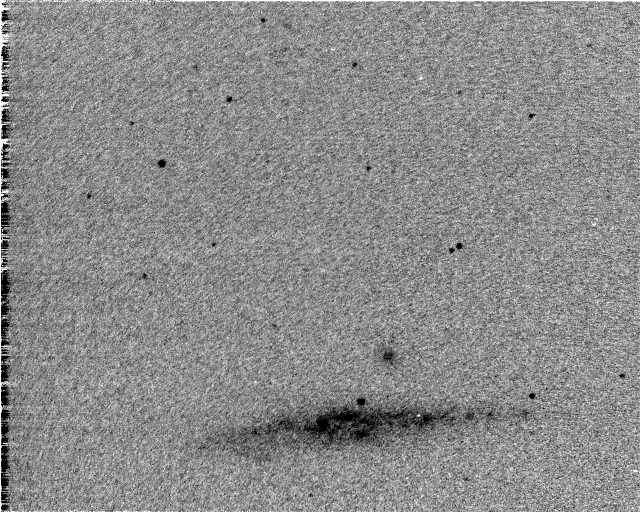
\includegraphics[width=\textwidth]{LSPR_annotated_images/Jul25Series1.png}
\end{figure}


\begin{center}
\begin{tabular}{| c |  c | c | c | c |  c | }
\hline
Star &  $x^{\text{star}}_{\text{pixel}}$ & $y^{\text{star}}_{\text{pixel}}$  & $\alpha_{\text{star}}$ &  $\delta_{\text{star}}$ \\ \hline \hline

\end{tabular}
\end{center}

%%%%%%%%%%%%%%%%%%%%%%%%%%%%%%%%%%%%%%%%%%%%%%%%%%%%%%%%%%%%%%%%%%%%%%

\clearpage
\section*{July 25, 2011}
\subsection{Series 2}
\begin{center}
\begin{tabular}{| c |  c | c | c | }
\hline
JD & UT & \# images & Filter \\ \hline
2455767.698177 & 04h 45m 21.9s & 5 & V-Filter \\ \hline
\end{tabular}
\end{center}

\begin{figure}[h!]
  \centering
   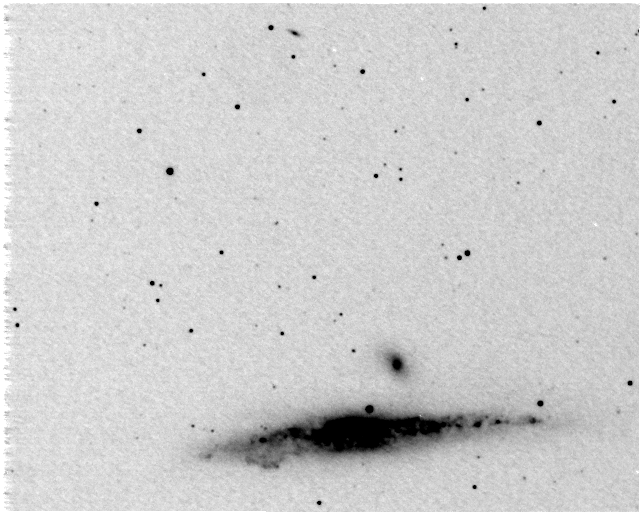
\includegraphics[width=\textwidth]{LSPR_annotated_images/Jul25Series2.png}
\end{figure}

Asteroid apparent magnitude $\approx$ 17.15

Image is even noisier than previous V-Filter series on July 16. This was unfortunately our last opportunity for photometry.

\begin{center}
\begin{tabular}{| c |  c | c | c | c |  c | }
\hline
Star & NOMAD Apparent Magnitude & Measured Apparent Magnitude \\ \hline \hline
UCAC3 246:109054 & 14.81 & Used for calibration \\ \hline
UCAC3 246:109059 & 16.21 & 16.03 \\ \hline
GSC 2531:1730 & 12.67 & 12.31 \\ \hline
\end{tabular}
\end{center}

%%%%%%%%%%%%%%%%%%%%%%%%%%%%%%%%%%%%%%%%%%%%%%%%%%%%%%%%%%%%%%%%%%%%%%
%%%%%%%%%%%%%%%%%%%%%%%%%%%%%%%%%%%%%%%%%%%%%%%%%%%%%%%%%%%%%%%%%%%%%%

\end{document}  